\documentclass[11pt,a4paper]{article}

\usepackage[margin=2.4cm]{geometry}
\usepackage[T1]{fontenc}
\usepackage[utf8]{inputenc}
\usepackage{lmodern}
\usepackage{microtype}
\usepackage{amsmath,amssymb,mathtools}
\usepackage{braket}
\usepackage{booktabs}
\usepackage{tabularx}
\usepackage{array}
\usepackage{enumitem}
\usepackage{graphicx}
\usepackage{caption}
\usepackage{listings}
\usepackage{tikz}
\usetikzlibrary{positioning,arrows.meta}
\usepackage[numbers,sort&compress]{natbib}
\usepackage{xcolor}
\usepackage[colorlinks=true,linkcolor=blue!50!black,citecolor=blue!50!black,urlcolor=blue!50!black]{hyperref}
\usepackage[capitalise,noabbrev]{cleveref}

\newcolumntype{Y}{>{\raggedright\arraybackslash}X}
\newcommand{\GW}{\textit{GW}}
\newcommand{\iDEA}{iDEA}
\newcommand{\code}[1]{\texttt{#1}}
\newcommand{\dx}{\delta x}
\newcommand{\mat}[1]{\mathsf{#1}}
\newcommand{\Tr}{\operatorname{Tr}}
\newcommand{\sgn}{\operatorname{sgn}}
\newcommand{\Nx}{N_x}
\newcommand{\up}{{\uparrow}}
\newcommand{\dn}{{\downarrow}}

\captionsetup{font=small,labelfont=bf}
\urlstyle{tt}
\setlist{itemsep=2pt,topsep=4pt}
\setlength{\emergencystretch}{2.5em}

\lstset{
  basicstyle=\ttfamily\footnotesize,
  columns=fullflexible,
  keepspaces=true,
  frame=single,
  framesep=4pt,
  rulecolor=\color{black!30},
  backgroundcolor=\color{black!3},
  xleftmargin=6pt,
  xrightmargin=6pt,
  breaklines=true,
  aboveskip=8pt,
  belowskip=8pt,
  showstringspaces=false,
}
\lstdefinestyle{python}{language=Python,keywordstyle=\color{blue!60!black},commentstyle=\color{green!40!black},stringstyle=\color{red!50!black}}
\lstdefinestyle{pseudo}{mathescape=true,morekeywords={for,each,in,if,else,return,until,repeat,end},keywordstyle=\bfseries}

% Generated by report/make_figures.py; do not edit.
\newcommand{\valTimeExact}{19}
\newcommand{\valNx}{61}
\newcommand{\valLength}{12}
\newcommand{\valDx}{0.40}
\newcommand{\valEzero}{-0.510834}
\newcommand{\valMu}{-0.2784}
\newcommand{\valHminus}{-0.0460}
\newcommand{\valEAffinity}{0.0460}
\newcommand{\valDimUp}{1{,}830}
\newcommand{\valDimDown}{3{,}721}
\newcommand{\valPolesUp}{1{,}831}
\newcommand{\valPolesDown}{3{,}721}
\newcommand{\valRayleigh}{7\times10^{-15}}
\newcommand{\valCompleteness}{1\times10^{-15}}
\newcommand{\valFirstMoment}{6\times10^{-14}}
\newcommand{\valGMError}{3\times10^{-16}}
\newcommand{\valSigmaXResidual}{1\times10^{-14}}
\newcommand{\valEGzWz}{-0.517064}
\newcommand{\valEpsGzWz}{-0.5165}
\newcommand{\valEGWz}{-0.516250}
\newcommand{\valEpsGWz}{-0.5150}
\newcommand{\valEGW}{-0.516269}
\newcommand{\valEpsGW}{-0.5138}
\newcommand{\valScreeningExact}{2\times10^{-17}}
\newcommand{\valScreeningGzWz}{1.7\times10^{-2}}
\newcommand{\valScreeningGWz}{1.7\times10^{-2}}
\newcommand{\valScreeningGW}{1.7\times10^{-2}}
\newcommand{\valDepthExactUp}{-0.0061}
\newcommand{\valDepthExactDown}{-0.0309}
\newcommand{\valDepthGWUp}{-0.0116}
\newcommand{\valDepthGWDown}{-0.0220}
\newcommand{\valKrylovDim}{4{,}410}


\title{\textbf{Exact one-body Green's functions and self-energies\\ from exact many-body states}\\[4pt]
\large Intuition, method, implementation and testing of the exact $G$ and $\Sigma_{xc}$ solver in \iDEA{}}
\author{Technical report accompanying the \iDEA{} pull request\\
\small \code{iDEA.methods.interacting.green\_function}, \code{iDEA.observables}, \code{iDEA.plotting}}
\date{October 2026}

\begin{document}
\maketitle

% ---------------------------------------------------------------------------
\begin{abstract}
\noindent
This report describes how \iDEA{} builds the \emph{exact} one-body Green's function $G(x,x';t\text{ or }\omega)$ and the \emph{exact} exchange-correlation self-energy $\Sigma_{xc}(x,x';t\text{ or }\omega)$ of an interacting electronic state. Both are built from the exact eigenstates of the $(N-1)$-, $N$- and $(N+1)$-electron systems.

\begin{itemize}
\item \textbf{The $N\pm1$ problems.} These are posed in an ordered Slater-determinant basis. They are solved either by complete diagonalisation or by a block Krylov method seeded with the states $\hat\psi^{(\dagger)}(x)\ket{\Psi_0}$. The block Krylov method reproduces the low-order moments of $G$ exactly. As a result, the sum rules and the static self-energy are exact even when the excitation spectrum is truncated.
\item \textbf{The self-energy.} It is obtained in closed pole form by Löwdin partitioning, carried out as a block Lanczos recursion on the poles of $G$. Each correlation pole carries a \emph{character} that fixes its time ordering.
\item \textbf{Evaluation.} The resulting objects can be evaluated in real time, at real or complex frequency, and on the imaginary axes used by the \GW{} code in \iDEA{}, so exact and \GW{} results can be compared directly. They can also be animated as videos of $G(x,x')$ and $\Sigma(x,x')$.
\end{itemize}

We explain the physical meaning of each element of $G$ and $\Sigma$, derive every step of the method, describe the code module by module, and list the tests. On every grid tested, the implementation satisfies all exact identities (completeness, density matrix, first moment, Galitskii--Migdal energy and Dyson's equation) to machine precision.

As an illustration, we compute the exact $G$ and $\Sigma_{xc}$ of the one-dimensional hydrogen atom. The exact self-energy annihilates the occupied orbital at every frequency. Self-consistent \GW{} instead leaves a self-screening residual of order $10^{-2}$.
\end{abstract}

\tableofcontents

% ===========================================================================
\section{Introduction}

The one-body Green's function $G$ is the central object of many-body perturbation theory~\cite{hedin1965,fetter1971,stefanucci2013,martin2016}. It contains:
\begin{itemize}
\item the ground-state density and density matrix;
\item the total energy, through the Galitskii--Migdal formula~\cite{galitskii1958};
\item the complete spectrum of electron addition and removal energies, i.e.\ photoemission and inverse photoemission.
\end{itemize}

The self-energy $\Sigma$ is defined by Dyson's equation as the difference between the inverse of $G$ and that of a simple reference. It is the non-local, energy-dependent potential that an added or removed electron feels. Approximations such as \GW{}~\cite{hedin1965} are approximations to $\Sigma$. Judging and improving them requires knowing what the exact $\Sigma$ looks like.

In real materials, the exact $\Sigma$ is out of reach. In one-dimensional model systems, the exact many-body states can be found numerically for a few electrons on a fine real-space grid. This is what \iDEA{} was built for~\cite{hodgson2013,hodgson2016,wetherell2018,wetherell2019}.

This report describes a new part of \iDEA{} that builds the \emph{exact} $G$ and \emph{exact} $\Sigma_{xc}$ from those states, with the full dependence on both positions $x$ and $x'$ and on time or frequency. To our knowledge, such exact two-point quantities have rarely been shown for real-space model systems. Being able to compute and \emph{watch} them, as videos of $G(x,x';t)$ or $\Sigma(x,x';\omega)$, has three uses:
\begin{itemize}
\item a benchmark for \GW{} and vertex corrections~\cite{romaniello2009,nelson2007,wetherell2018};
\item a direct test of the nearsightedness of the self-energy~\cite{kohn1996,prodan2005,wetherell2019}, which is the subject of the accompanying research proposal;
\item a teaching tool.
\end{itemize}

The report is organised as follows:
\begin{itemize}
\item \Cref{sec:background} explains what each element of $G$ and $\Sigma$ means physically.
\item \Cref{sec:method} derives the method.
\item \Cref{sec:implementation} describes the code.
\item \Cref{sec:testing} describes the tests.
\item \Cref{sec:results} shows illustrative results for the one-dimensional hydrogen atom.
\item \Cref{sec:limitations} lists limitations and next steps.
\item \Cref{app:production} gives the production calculations to run on a GPU.
\item \Cref{app:derivations} collects derivations.
\end{itemize}

Hartree atomic units are used throughout.

% ===========================================================================
\section{Background and intuition}
\label{sec:background}

\subsection{The Green's function: propagation of an added electron or hole}

For a state $\ket{\Psi_0}$ of energy $E_0$, the time-ordered Green's function of spin channel $\sigma$ is
\begin{equation}
G_\sigma(x,x';t) = -i\braket{\Psi_0|\mathcal{T}\,\hat\psi_\sigma(x,t)\,\hat\psi_\sigma^\dagger(x',0)|\Psi_0},
\label{eq:G}
\end{equation}
where $\hat\psi_\sigma(x,t) = e^{i\hat Ht}\hat\psi_\sigma(x)e^{-i\hat Ht}$.

\paragraph{Positive times: an added electron.} For $t>0$,
\begin{equation}
iG(x,x';t) = \braket{\Psi_0|\hat\psi(x)\,e^{-i(\hat H-E_0)t}\,\hat\psi^\dagger(x')|\Psi_0}.
\end{equation}
In words:
\begin{enumerate}
\item add an electron at $x'$;
\item let the whole interacting $(N+1)$-electron system evolve for a time $t$;
\item project onto the state in which an electron has been added at $x$ to the undisturbed ground state.
\end{enumerate}
A column $G(\cdot,x_0;t)$ is therefore the wavefunction of an electron injected at $x_0$, dressed by the response of all the others.

\paragraph{Negative times: a hole.} For $t<0$, the same holds for a hole: an electron removed, as in photoemission.

\paragraph{Equal times: the density matrix.} The equal-time limit from below is the one-body density matrix,
\begin{equation}
G_\sigma(x,x';0^-) = i\gamma_\sigma(x,x'), \qquad \gamma_\sigma(x,x') = \braket{\Psi_0|\hat\psi_\sigma^\dagger(x')\hat\psi_\sigma(x)|\Psi_0}.
\label{eq:density-matrix}
\end{equation}
\begin{itemize}
\item Its diagonal is the spin density, $n_\sigma(x) = \gamma_\sigma(x,x)$. This is the precise sense in which the density is the diagonal of $G$.
\item Off the diagonal, $\gamma(x,x')$ is the coherence between removing an electron at $x$ and removing it at $x'$. It determines the kinetic energy, the exchange energy and the momentum distribution.
\item How fast $\gamma$ decays with $|x-x'|$ is one measure of nearsightedness~\cite{kohn1996,prodan2005}.
\end{itemize}

\subsection{Lehmann representation, Dyson orbitals and the spectral function}

Inserting complete sets of $(N\pm1)$-electron eigenstates into \cref{eq:G} gives the Lehmann representation~\cite{lehmann1954,fetter1971}:
\begin{equation}
G_\sigma(x,x';z) = \sum_k \frac{d_k(x)\,d_k^*(x')}{z-\varepsilon_k}.
\label{eq:lehmann}
\end{equation}
There are two kinds of pole:
\begin{itemize}
\item \textbf{Removal poles,} $\varepsilon_k = E_0 - E^{N-1}_k$, with Dyson orbitals $d_k(x) = \braket{\Psi^{N-1}_k|\hat\psi_\sigma(x)|\Psi_0}$.
\item \textbf{Addition poles,} $\varepsilon_k = E^{N+1}_k - E_0$, with Dyson orbitals $d_k(x) = \braket{\Psi_0|\hat\psi_\sigma(x)|\Psi^{N+1}_k}$.
\end{itemize}
The poles are the energies measured in photoemission ($-\varepsilon_k$ is an ionisation energy) and inverse photoemission. Each Dyson orbital is the wavefunction of the electron removed or added, and its norm is the spectroscopic factor or quasiparticle weight.

\paragraph{Time and frequency forms.} The time-ordered function is
\begin{equation}
G(x,x';t) = -i\sum_k d_k(x)d_k^*(x')\,e^{-i\varepsilon_k t}\big[\theta(t)(1-f_k) - \theta(-t)f_k\big],
\label{eq:G-time}
\end{equation}
where $f_k=1$ for removal and $f_k=0$ for addition poles. In frequency, it is \cref{eq:lehmann} with $z = \omega + i\eta$ for addition poles and $z = \omega - i\eta$ for removal poles, $\eta\to0^+$.

\paragraph{The spectral function.} It is
\begin{equation}
A(x,x';\omega) = \sum_k d_k(x)d_k^*(x')\,\delta(\omega-\varepsilon_k).
\end{equation}
Its diagonal, $A(x,x;\omega)$, is the local density of states for adding or removing an electron of energy $\omega$ at $x$, which is what a scanning-tunnelling microscope measures.

\paragraph{Sum rules.} The anticommutation relations and the Hamiltonian give exact sum rules:
\begin{align}
\int A(x,x';\omega)\,d\omega &= \delta(x-x') &&\text{(completeness)},\label{eq:completeness}\\
\int_{-\infty}^{\mu} A(x,x';\omega)\,d\omega &= \gamma(x,x') &&\text{(density matrix)},\\
\int \omega\,A(x,x';\omega)\,d\omega &= h_\infty(x,x') &&\text{(first moment)},\label{eq:first-moment}\\
E_0 &= \tfrac12\sum_\sigma\sum_{m\in\text{removal}}\braket{d_m|\hat h_0+\varepsilon_m|d_m} &&\text{(Galitskii--Migdal)}.\label{eq:gm}
\end{align}
The first-moment matrix is the static Hamiltonian
\begin{equation}
h_\infty(x,x') = h_0(x,x') + v_H(x)\delta(x-x') + \Sigma_{x\sigma}(x,x'),
\qquad
\Sigma_{x\sigma}(x,x') = -\gamma_\sigma(x,x')\,v(x,x'),
\label{eq:hinf}
\end{equation}
where $h_0 = -\tfrac12\partial_x^2 + v_\text{ext}$, $v_H$ is the Hartree potential of the total density, and $\Sigma_x$ is the Fock operator of the \emph{exact} density matrix (\cref{app:first-moment}).

\subsection{The self-energy: the potential felt by the added or removed electron}

The exchange-correlation self-energy is defined by Dyson's equation,
\begin{equation}
G^{-1}(z) = z - h_0 - v_H - \Sigma_{xc}(z), \qquad \Sigma_{xc}(z) = \Sigma_x + \Sigma_c(z).
\label{eq:dyson}
\end{equation}

\paragraph{The quasiparticle equation.} Because $G^{-1}(\varepsilon_k)\,d_k = 0$, the Dyson orbitals satisfy the quasiparticle equation exactly:
\begin{equation}
\big[h_0 + v_H\big]d_k(x) + \int\Sigma_{xc}(x,x';\varepsilon_k)\,d_k(x')\,dx' = \varepsilon_k\,d_k(x).
\label{eq:qp}
\end{equation}
So $\Sigma_{xc}$ plays the role that the Kohn--Sham $v_{xc}$ plays for Kohn--Sham orbitals~\cite{godby1988}, with two differences:
\begin{itemize}
\item it is \emph{non-local}: the element $(x,x')$ moves amplitude from $x'$ to $x$;
\item it depends on \emph{energy}: an electron added at a different energy feels a different potential.
\end{itemize}

\paragraph{The static part.} Expanding \cref{eq:lehmann} at large $z$ gives $G(z) = z^{-1} + h_\infty z^{-2} + O(z^{-3})$. Hence $G^{-1}(z) = z - h_\infty + O(z^{-1})$, and
\begin{equation}
\Sigma_{xc}(z\to\infty) = \Sigma_x .
\end{equation}
The static part of the exact self-energy is the Fock operator built from the exact density matrix. It is instantaneous in time, carries Pauli exclusion and the self-interaction correction, and has the spatial range of $\gamma$.

\paragraph{The correlation part.} The correlation part has poles,
\begin{equation}
\Sigma_c(x,x';z) = \sum_p \frac{r_p(x)\,r_p^*(x')}{z-\zeta_p}.
\label{eq:sigma-poles}
\end{equation}
Each part has a physical reading:
\begin{itemize}
\item \textbf{Poles $\zeta_p$.} These are the energies at which the added or removed electron can hand energy to the rest of the system by exciting it (two-particle--one-hole and two-hole--one-particle configurations, or shake-up). They produce satellites in $A(\omega)$ and take weight away from the quasiparticle peaks.
\item \textbf{Residues $r_p(x)$.} These say how strongly an electron at $x$ couples into each such channel.
\item \textbf{$\mathrm{Re}\,\Sigma_c$.} This is the relaxation and polarisation energy.
\item \textbf{$-\mathrm{Im}\,\Sigma_c^R(x,x;\omega)\ge0$.} This acts like a local absorbing potential: the rate at which an electron added with energy $\omega$ leaks out of the one-particle channel.
\item \textbf{$\Sigma_c(x,x';t)$ in real time.} This is a memory kernel: the amplitude for the electron to leave the one-particle channel at $x'$ (by exciting the others) and to return at $x$ a time $t$ later. In \GW{}, $\Sigma = iGW$: the electron interacts with the polarisation it has left behind.
\end{itemize}

\subsection{One electron: no self-interaction, and \GW{} self-screening}
\label{sec:one-electron}

For a single spin-up electron in the orbital $\phi$, with $\hat h_0\phi = E_0\phi$, the structure is very simple.

\paragraph{The removal part.} The only $(N-1)$-electron state is the vacuum. So $G_\up$ has a single removal pole, at $\varepsilon = E_0$, with Dyson orbital $\phi$ and weight one. By completeness (\cref{eq:completeness}), all addition Dyson orbitals lie in the orthogonal complement of $\phi$. Therefore $G_\up(z) = \phi\phi^*/(z-E_0) \oplus G_\text{add}(z)$, and $G_\up^{-1}(z)\phi = (z-E_0)\phi$ at every $z$.

\paragraph{The self-energy.} Inserting this into \cref{eq:dyson} with $\hat h_0\phi = E_0\phi$ gives
\begin{equation}
\big[v_H + \Sigma_{xc\up}(z)\big]\phi = 0 \quad\text{for all } z.
\end{equation}
The exchange part does this alone, since $\Sigma_{x\up}\phi = -v_H\phi$ when $\gamma_\up = \phi\phi^*$. So the correlation part must annihilate the orbital: $\Sigma_{c\up}(z)\phi = 0$. The exact self-energy has no self-interaction at any frequency.

\paragraph{The \GW{} self-energy.} The \GW{} self-energy $iGW$ contains the electron's own orbital in $G$, and $W$ screens the electron by its own density. This leaves $\Sigma_c^{\GW}\phi\ne0$: the electron screens itself. This self-screening error was identified in the hydrogen atom by Nelson \emph{et al.}~\cite{nelson2007} and analysed with \iDEA{} in Ref.~\cite{wetherell2018}.

\paragraph{Spin down.} In the spin-down channel, $G_\dn$ has no removal part at all, $\gamma_\dn = 0$ and $\Sigma_{x\dn} = 0$. So $\Sigma_\dn = \Sigma_{c\dn}$ is pure correlation: it describes how an added spin-down electron polarises the bound spin-up electron. This is the physics that binds the H$^-$ ion.

% ===========================================================================
\section{Method}
\label{sec:method}

\subsection{Discretisation and second quantisation on the grid}

\paragraph{The grid and field operators.} \iDEA{} represents states on a uniform grid $x_i$, $i=1,\dots,\Nx$, with spacing $\dx$. We define dimensionless fermion operators
\begin{equation}
c_{i\sigma} = \sqrt{\dx}\,\hat\psi_\sigma(x_i), \qquad \{c_{i\sigma},c^\dagger_{j\sigma'}\} = \delta_{ij}\delta_{\sigma\sigma'}.
\end{equation}

\paragraph{Kernels and matrices.} Two-point quantities are stored as \emph{kernels} $A(x_i,x_j)$, which act as $\int A(x,x')f(x')\,dx' \to \sum_j A(x_i,x_j)f(x_j)\,\dx$. The matrix that acts on discrete vectors is therefore $\mat A = A\,\dx$. This is the convention of the \GW{} module \code{iDEA.methods.mbpt}~\cite{rojas1995,rieger1999}, and it is used throughout.

\paragraph{The Hamiltonian.} It is
\begin{equation}
\hat H = \sum_{ij\sigma}(\mat h_0)_{ij}\,c^\dagger_{i\sigma}c_{j\sigma} + \frac12\sum_{ij\sigma\sigma'} v_{ij}\,c^\dagger_{i\sigma}c^\dagger_{j\sigma'}c_{j\sigma'}c_{i\sigma},
\end{equation}
\begin{itemize}
\item $\mat h_0$ is the finite-difference kinetic-energy stencil plus $\mathrm{diag}(v_\text{ext})$;
\item $v_{ij} = v(x_i,x_j)$ is the (softened) interaction.
\end{itemize}

\paragraph{The many-body state.} An \iDEA{} many-body state stores the full antisymmetric wavefunction $\Psi(x_1\sigma_1,\dots,x_N\sigma_N)$, normalised as $\sum|\Psi|^2\dx^N=1$. We work with the \emph{spin-ordered} spatial wavefunction, with all $N_\up$ spin-up electrons first:
\begin{equation}
\psi(x_1,\dots,x_{N_\up};y_1,\dots,y_{N_\dn}) = \sqrt{\tbinom{N}{N_\up}}\;\dx^{N/2}\;\Psi(x_1{\up},\dots,x_{N_\up}{\up},y_1{\dn},\dots,y_{N_\dn}{\dn}).
\label{eq:spin-ordered}
\end{equation}
It is antisymmetric within each spin group and normalised as $\sum|\psi|^2=1$ (\cref{app:spin-ordered}). The code checks this normalisation and raises an error if it fails.

\subsection{Sector Hamiltonians in an ordered Slater-determinant basis}
\label{sec:sectors}

The $(N\pm1)$-electron problems are solved in \emph{sectors} with fixed numbers $(n_\up,n_\dn)$ of up and down electrons.

\paragraph{The determinant basis.} A sector is spanned by the ordered determinants
\begin{equation}
\ket{\mathbf a;\mathbf b} = c^\dagger_{a_1\up}\cdots c^\dagger_{a_{n_\up}\up}\,c^\dagger_{b_1\dn}\cdots c^\dagger_{b_{n_\dn}\dn}\ket{0}, \qquad a_1<\dots<a_{n_\up},\quad b_1<\dots<b_{n_\dn}.
\end{equation}
Sites are labelled $0,\dots,\Nx-1$. The combinations are enumerated in colexicographic order, so the position of a combination in the list equals its rank in the combinatorial number system:
\begin{equation}
r(\mathbf a) = \sum_{j=1}^{n}\binom{a_j}{j}.
\label{eq:rank}
\end{equation}
The determinant $\ket{\mathbf a;\mathbf b}$ has index $r(\mathbf a)\binom{\Nx}{n_\dn} + r(\mathbf b)$. Looking up the index of any determinant is therefore a vectorised sum over a precomputed table of binomial coefficients; no dictionaries or searches are needed.

\paragraph{Coefficients of a state.} For a state with spin-ordered wavefunction $\psi$,
\begin{equation}
\braket{\mathbf a;\mathbf b|\Psi} = \sqrt{n_\up!\,n_\dn!}\;\psi(\mathbf a;\mathbf b).
\end{equation}

\paragraph{The isometry $P$.} The existing \iDEA{} Hamiltonian acts on the spatial product space $\mathbb{R}^{\Nx^N}$ (C order, axis $k$ for electron $k$). To reuse it unchanged, we build the sparse isometry $P$ from the determinant basis into the product space. Column $(\mathbf a,\mathbf b)$ of $P$ is
\begin{equation}
P\,e_{(\mathbf a,\mathbf b)} = \frac{1}{\sqrt{n_\up!\,n_\dn!}}\sum_{\pi\in S_{n_\up}}\sum_{\rho\in S_{n_\dn}}\sgn(\pi)\sgn(\rho)\;e_{(a_{\pi(1)},\dots,a_{\pi(n_\up)},\,b_{\rho(1)},\dots,b_{\rho(n_\dn)})},
\end{equation}
which satisfies $P^\top P = 1$. The sector Hamiltonian is then
\begin{equation}
\mat H_D = P^\top\,\mat H_\text{prod}\,P,
\end{equation}
where $\mat H_\text{prod}$ is \code{interacting.hamiltonian} for a system with the same grid, potentials and stencil, and electrons \code{'u'*n\_up + 'd'*n\_dn}.

\paragraph{Dimensions.} The sector has dimension $D = \binom{\Nx}{n_\up}\binom{\Nx}{n_\dn}$, about $n_\up!\,n_\dn!$ times smaller than $\Nx^N$. \Cref{tab:dimensions} lists the sizes that matter here. The vacuum sector is handled separately: its energy is $0$ and its only state is $\ket{0}$.

\begin{table}[t]
\centering\small
\caption{Dimensions of the $(N\pm1)$-electron sectors. Hydrogen ($N=1$, spin up) needs the vacuum and the sectors $(2,0)$ and $(1,1)$. A two-electron atom ($N_\up=N_\dn=1$) needs $(0,1)$, $(1,0)$, $(2,1)$ and $(1,2)$.}
\label{tab:dimensions}
\begin{tabular}{lrrrr}
\toprule
system & $\Nx$ & sector & $D$ & product space $\Nx^{N\pm1}$ \\
\midrule
hydrogen & 61 & $(2,0)$ & 1\,830 & 3\,721 \\
hydrogen & 61 & $(1,1)$ & 3\,721 & 3\,721 \\
hydrogen & 151 & $(2,0)$ & 11\,325 & 22\,801 \\
hydrogen & 151 & $(1,1)$ & 22\,801 & 22\,801 \\
two electrons & 21 & $(2,1)$ & 4\,410 & 9\,261 \\
two electrons & 41 & $(2,1)$ & 33\,620 & 68\,921 \\
two electrons & 101 & $(2,1)$ & 510\,050 & 1\,030\,301 \\
\bottomrule
\end{tabular}
\end{table}

\subsection{Field operators and Jordan--Wigner signs}
\label{sec:field-operators}

\paragraph{Action on determinants.} With the operator ordering above (all up operators to the left of all down operators), the annihilation operators act on a determinant as follows~\cite{jordan1928}:
\begin{equation}
c_{i\up}\ket{\mathbf a;\mathbf b} = (-1)^{k-1}\ket{\mathbf a\setminus a_k;\mathbf b}\ \ (i=a_k),\qquad
c_{i\dn}\ket{\mathbf a;\mathbf b} = (-1)^{n_\up+k-1}\ket{\mathbf a;\mathbf b\setminus b_k}\ \ (i=b_k),
\label{eq:jordan-wigner}
\end{equation}
and give zero if site $i$ is empty. The creation operators are the adjoints.

\paragraph{Source vectors.} We need the $\Nx$ removal sources $g_i = c_{i\sigma}\ket{\Psi}$, which lie in the $(N-1)$ sector, and the $\Nx$ addition sources $f_i = c^\dagger_{i\sigma}\ket{\Psi}$, which lie in the $(N+1)$ sector. All of them are built at once:
\begin{enumerate}
\item Loop over the slot $k$ in the larger of the two sectors.
\item For every determinant of that sector at once, delete slot $k$ and find the rank of the smaller determinant from \cref{eq:rank}.
\item Scatter the signed coefficient into the column for site $i = a_k$ (or $b_k$).
\end{enumerate}
The product space is never used.

\paragraph{Checks.} Two identities check the signs and the normalisation:
\begin{equation}
\braket{g_i|g_j} = \gamma(x_j,x_i)\,\dx, \qquad \braket{f_i|f_j} = \delta_{ij} - \gamma(x_i,x_j)\,\dx.
\label{eq:source-identities}
\end{equation}

\subsection{Lehmann poles}

Each sector is diagonalised as $\mat H_D = \sum_n E_n\ket{n}\bra{n}$.

\paragraph{Discrete Dyson amplitudes.} These are:
\begin{itemize}
\item removal: $\varepsilon_n = E_0 - E_n$ and $\mat V_{in} = \braket{n|g_i}$;
\item addition: $\varepsilon_n = E_n - E_0$ and $\mat V_{in} = \braket{n|f_i}^*$.
\end{itemize}
With these,
\begin{equation}
\mat G_{ij}(z) = \sum_n\frac{\mat V_{in}\mat V_{jn}^*}{z-\varepsilon_n}, \qquad d_n(x_i) = \mat V_{in}/\sqrt{\dx}.
\end{equation}

\paragraph{Practical details.}
\begin{itemize}
\item \textbf{Unreachable states.} States with total weight $\sum_i|\mat V_{in}|^2<10^{-14}$ cannot be reached by the field operator (for example, because of symmetry) and are dropped.
\item \textbf{The ground-state energy.} $E_0$ is recomputed as a Rayleigh quotient in the determinant basis, and its residual $\Vert(\mat H_D-E_0)\Psi\Vert$ is checked: the code raises an error above $10^{-6}$ and warns above $10^{-8}$. This stops the tolerance of the $N$-electron eigensolver from shifting every pole.
\item \textbf{The chemical potential.} A single $\mu = \tfrac12(\min\varepsilon^+ + \max\varepsilon^-)$, at the centre of the gap over both spin channels, is used for the imaginary axis. It is \code{None} when there is no gap; for example, the lowest triplet state of a two-electron atom is an excited state with $\varepsilon^+<\varepsilon^-$.
\item \textbf{Derived quantities.} The density matrix $\gamma_\sigma = \sum_\text{removal}d\,d^*$, the density, the Hartree potential and the Galitskii--Migdal energy (\cref{eq:gm}) follow directly from the poles.
\end{itemize}

\subsection{Large sectors: block Krylov with exact moments}
\label{sec:krylov}

Complete diagonalisation costs $O(D^3)$ time and $O(D^2)$ memory. Sectors larger than \code{dense\_max} (default $6000$) are therefore treated with a block Krylov (block Rayleigh--Ritz) method seeded with the sources $\mat B = [g_1,\dots,g_{\Nx}]$ or $[f_1,\dots,f_{\Nx}]$~\cite{golub1977,dagotto1994}.

\paragraph{Building the basis.} An orthonormal basis $\mat Q$ of
\begin{equation}
\mathcal K_m(\mat H_D,\mat B) = \mathrm{span}\{\mat B,\mat H_D\mat B,\dots,\mat H_D^{m-1}\mat B\}
\end{equation}
is built block by block:
\begin{itemize}
\item The first block is the left singular vectors of $\mat B$ whose singular values exceed $\tau\,\sigma_\text{max}$.
\item Each new block $\mat W = \mat H_D\mat Q_\text{last}$ is orthogonalised against all previous vectors by classical Gram--Schmidt applied twice (CGS2, which keeps orthogonality at the level of the unit round-off~\cite{giraud2005}).
\item The new block is then deflated by a thin SVD, keeping directions with singular values above $\tau\Vert\mat H_D\Vert_\infty$ (default $\tau=10^{-10}$).
\end{itemize}
The recursion stops when \code{krylov\_dim} vectors are reached (default $30\Nx$) or when the space is exhausted.

\paragraph{The approximate poles.} The projected matrix $\mat T = \mat Q^\dagger\mat H_D\mat Q$ (symmetrised) is diagonalised, $\mat T = \mat Y\Theta\mat Y^\dagger$. The Ritz values $\Theta$ give the poles and $\mat Y^\dagger\mat Q^\dagger\mat B$ the amplitudes.

\paragraph{Theorem (moment preservation).} \emph{For every $k\le 2m-1$, $\mat B^\dagger\mat H_D^k\mat B = \mat B^\dagger\mat Q\,\mat T^k\,\mat Q^\dagger\mat B$.}

\emph{Proof.} Let $\Pi=\mat Q\mat Q^\dagger$. For $j\le m-1$, $\mat H_D^j\mat B\in\mathcal K_m$, and by induction $\mat Q\mat T^j\mat Q^\dagger\mat B = \Pi\mat H_D\Pi\mat H_D^{j-1}\mat B = \Pi\mat H_D^j\mat B = \mat H_D^j\mat B$. Write $k=a+c+b$ with $a,b\le m-1$ and $c\in\{0,1\}$. Then
\[
\mat B^\dagger\mat H_D^k\mat B = (\mat H_D^a\mat B)^\dagger\mat H_D^c(\mat H_D^b\mat B) = \mat B^\dagger\mat Q\mat T^a(\mat Q^\dagger\mat H_D^c\mat Q)\mat T^b\mat Q^\dagger\mat B = \mat B^\dagger\mat Q\mat T^k\mat Q^\dagger\mat B. \qquad\square
\]

\paragraph{Consequences.} The moments of the Krylov approximation to $G$, $\sum_n\mat V_n\mat V_n^\dagger\varepsilon_n^k$, are polynomials of degree $k$ in $\mat H_D$, so they are exact for $k\le 2m-1$. This is the matrix form of Gauss quadrature~\cite{golub2010}. Three things follow:
\begin{enumerate}
\item Completeness ($k=0$) and the first moment ($k=1$) are exact for \emph{any} truncation.
\item So the static self-energy $\Sigma_x$ (\cref{eq:hinf}) is exact for any truncation too.
\item Truncation moves only the high-lying poles, and the pole spectrum converges as $m$ grows. All poles are exact once the space is exhausted.
\end{enumerate}
\Cref{fig:krylov} demonstrates this. The same moment-conserving idea underlies the block-Lanczos treatment of self-energies in auxiliary second-order Green's function methods~\cite{backhouse2020}.

\paragraph{GPU.} With \code{GPU=True}, the dense diagonalisation (\code{cupy.linalg.eigh}) and the Krylov recursion (CuPy sparse matrix products, CGS2 and SVD) run on the GPU. The results are copied back to the host.

\begin{figure}[t]
\centering
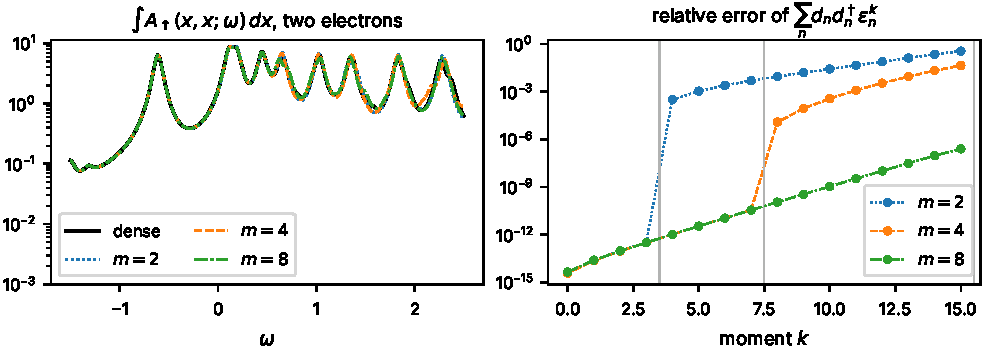
\includegraphics[width=\textwidth]{figures/krylov_convergence.pdf}
\caption{Block Krylov against complete diagonalisation for a two-electron atom ($v_\text{ext}=-2/(|x|+1)$, $\Nx=21$; the $(N+1)$ sectors have dimension \valKrylovDim). Left: the spectral function converges as the number of blocks $m$ grows. Right: the moments $\sum_n d_nd_n^\dagger\varepsilon_n^k$ are exact to machine precision for every $k\le 2m-1$ (grey lines), as the theorem of \cref{sec:krylov} guarantees.}
\label{fig:krylov}
\end{figure}

\subsection{The exact self-energy in pole form}
\label{sec:self-energy}

Collect the poles of one spin channel in $\mat E=\mathrm{diag}(\varepsilon_1,\dots,\varepsilon_M)$ and the discrete amplitudes in $\mat V\in\mathbb C^{\Nx\times M}$. Then $\mat G(z) = \mat V(z-\mat E)^{-1}\mat V^\dagger$, and completeness says $\mat V\mat V^\dagger = 1$. Numerically this holds to about $10^{-15}$; a symmetric re-orthonormalisation $\mat V\leftarrow(\mat V\mat V^\dagger)^{-1/2}\mat V$ makes it exact without changing the span.

\paragraph{Löwdin partitioning.} Complete the rows of $\mat V$ to a unitary matrix $\mat U = \begin{psmallmatrix}\mat V\\ \mat W\end{psmallmatrix}$ and set $\mat A = \mat U\mat E\mat U^\dagger$. Then $\mat G(z) = [(z-\mat A)^{-1}]_{11}$, and the Schur complement (Löwdin partitioning~\cite{lowdin1962}) gives
\begin{equation}
\mat G^{-1}(z) = z - \mat A_{11} - \mat A_{12}(z-\mat A_{22})^{-1}\mat A_{21}.
\end{equation}
Comparing with \cref{eq:dyson}:
\begin{equation}
\mat A_{11} = \mat V\mat E\mat V^\dagger = \mat h_0 + \mathrm{diag}(v_H) + \Sigma_x\dx, \qquad \Sigma_c(z)\,\dx = \mat A_{12}(z-\mat A_{22})^{-1}\mat A_{21}.
\label{eq:partition}
\end{equation}
The self-energy does not depend on how the complement $\mat W$ is chosen.

\paragraph{Block Lanczos on the poles.} We choose the completion by block Lanczos on the diagonal matrix $\mat E$, starting from the orthonormal block $\mat V^\dagger$. This is the routine of \cref{sec:krylov} applied to $\mat E$, which costs $O(M)$ per vector. It produces a block-tridiagonal $\mat T = \mat Q^\dagger\mat E\mat Q$ in which:
\begin{itemize}
\item the first diagonal block is $h_\infty\dx$, so that $\Sigma_x = (h_\infty\dx - \mat h_0 - \mathrm{diag}(v_H))/\dx$;
\item only the second block couples to the first.
\end{itemize}
Directions of $\mathbb C^M$ outside the Krylov space are invariant under $\mat E$ and orthogonal to $\mat V^\dagger$. They do not couple to the grid and are dropped exactly.

\paragraph{The poles of $\Sigma_c$.} Diagonalising the remaining block, $\mat T_{22} = \mat Z\,\mathrm{diag}(\zeta)\,\mat Z^\dagger$, gives \cref{eq:sigma-poles} with
\begin{equation}
r_p = \mat T_{12}\mat Z_{:,p}/\sqrt{\dx}.
\end{equation}
A spin channel with $M$ poles of $G$ therefore has at most $M-\Nx$ poles of $\Sigma_c$.

\paragraph{The check on the first block.} The first block is checked against the Fock operator of the density matrix computed independently from the removal poles (\cref{eq:hinf}). The largest deviation is stored in \code{info} as the first-moment error. A QR-based completion of $\mat V$ is kept in the tests as an independent reference for \cref{eq:partition}.

\subsection{Time ordering of the self-energy poles}
\label{sec:character}

The time-ordered $G$ assigns $+i\eta$ to addition poles and $-i\eta$ to removal poles: $\mat G^T(\omega) = \mat V(\omega-\mat E+i\eta\mat S)^{-1}\mat V^\dagger$, with $\mat S = \mathrm{diag}(\pm1)$. Repeating the partition with the same $\mat U$, to first order in $\eta$, replaces $\mat A_{22}$ by $\mat A_{22}-i\eta\,\mat W\mat S\mat W^\dagger$. First-order perturbation theory for the pole $\zeta_p$ then gives
\begin{equation}
\zeta_p \to \zeta_p - i\eta\,s_p, \qquad s_p = \sum_n S_n\,|\mat Y_{np}|^2\in[-1,1], \qquad \mat Y = \mat Q_{\ge2}\mat Z.
\end{equation}
\begin{itemize}
\item \textbf{The character.} $s_p$ is the weight of the pole on addition poles of $G$ minus its weight on removal poles. A pole is particle-like (it carries $+i\eta$ and $\theta(t)$) if $s_p>0$, and hole-like if $s_p<0$.
\item \textbf{Degenerate poles.} Within degenerate clusters of $\zeta$, the basis that diagonalises $\mat S$ is chosen first, as in degenerate perturbation theory.
\item \textbf{Ambiguous poles.} If $|s_p|<10^{-6}$, the time ordering is not determined at first order. This happens when a pole is built equally from addition and removal poles. The code warns and breaks the tie by the position of $\zeta_p$ relative to $\mu$.
\end{itemize}

\paragraph{Why not use $\zeta$ versus $\mu$.} The more familiar rule, retarded above $\mu$ and advanced below, holds for the continuous spectra of extended systems. It is \emph{not} reliable for the discrete in-gap poles of finite systems: in a randomised test during development it gave the wrong ordering for 348 of 4780 in-gap poles. The character rule is checked against Dyson inversion of the time-ordered $G$ in the tests (\cref{sec:testing}).

\paragraph{Imaginary time.} On the imaginary-time axis, the pole position relative to $\mu$ is used instead, following the \GW{} module. There, a decaying representation requires it.

\subsection{Evaluation on time and frequency axes}
\label{sec:axes}

\paragraph{The pole factors.} Given poles $\varepsilon_n$ with particle weights $f^+_n\in\{0,1\}$, the code evaluates $\sum_n d_n d_n^\dagger F_n$ with the factors $F_n$ of \cref{tab:axes}. The same table serves $G$ (using its occupations) and $\Sigma_c$ (using the characters).

\paragraph{Conventions at equal time.} The equal-time limit is taken as $t=0^-$, so that $G(t{=}0)=i\gamma$ and $G(\tau{=}0)=\gamma$. These are the conventions of \code{iDEA.methods.mbpt}, so exact and \GW{} quantities can be laid on the same grids.

\paragraph{Other quantities.}
\begin{itemize}
\item \textbf{The spectral function} is evaluated directly as a sum of Lorentzians of width $\eta$.
\item \textbf{Dyson inversion.} \code{self\_energy(..., method="dyson")} inverts \cref{eq:dyson} at each frequency, $\Sigma_{xc} = [w - \mat h_0 - \mathrm{diag}(v_H) - (\mat G\dx)^{-1}]/\dx$. This gives an independent check of the pole form.
\item \textbf{The Galitskii--Migdal energy} uses \cref{eq:gm}.
\end{itemize}

\begin{table}[t]
\centering\small
\caption{Pole factors $F_n$ on each axis, as implemented in \code{observables.\_pole\_factors}. Here $f_n^+ = 1$ for particle-like poles (addition poles of $G$; $s_p>0$ for $\Sigma_c$) and $0$ otherwise.}
\label{tab:axes}
\begin{tabularx}{\textwidth}{l>{\raggedright\arraybackslash}p{4.2cm}Y}
\toprule
axis & meaning & factor $F_n$ \\
\midrule
\code{t} & real time, time-ordered & $-ie^{-i\varepsilon_nt}\,[\theta(t)f^+_n - \theta(-t)(1-f^+_n)]$ \\
\code{t} & real time, retarded / advanced & $-ie^{-i\varepsilon_nt}\theta(t)$ \ / \ $ie^{-i\varepsilon_nt}\theta(-t)$ \\
\code{omega} & real frequency, time-ordered & $f^+_n/(\omega-\varepsilon_n+i\eta) + (1-f^+_n)/(\omega-\varepsilon_n-i\eta)$ \\
\code{omega} & real frequency, retarded / advanced & $1/(\omega-\varepsilon_n\pm i\eta)$ \\
\code{z} & complex frequency & $1/(z-\varepsilon_n)$ \\
\code{nu} & imaginary frequency about $\mu$ & $1/(\mu+i\nu-\varepsilon_n)$ \\
\code{tau} & imaginary time & $-f^+_ne^{-|\varepsilon_n-\mu|\tau}$ for $\tau>0$; \ $(1-f^+_n)e^{-|\varepsilon_n-\mu||\tau|}$ for $\tau\le0$ \\
\bottomrule
\end{tabularx}
\end{table}

\subsection{Visualisation}
\label{sec:visualisation}

\code{iDEA.plotting} draws any two-point quantity $A(x,x')$ as side-by-side heatmaps of its real, imaginary, absolute and phase parts, and animates it over the axis.

\paragraph{Colour scales.} The scale is fixed across all frames. By default it is the 99.5th percentile of the magnitude over the whole video, linear or symmetric-logarithmic, and symmetric about zero for real and imaginary parts. A strip under the heatmaps can show a one-dimensional trace with a moving marker:
\begin{itemize}
\item $\Tr A(\omega)$ for real-frequency $G$;
\item $|\Tr G(t)|$ for real-time $G$;
\item $\mathrm{Re}\,\Tr\Sigma$ for the self-energy.
\end{itemize}
Videos are written as \code{.mp4} (FFmpeg) or \code{.gif} (Pillow).

\paragraph{Visual aids for real time.} A point source $c_i^\dagger\ket{\Psi}$ excites every energy on the grid, up to $\sim 2/\dx^2$, so real-time quantities are dominated by fast grid modes. Two optional aids make real-time videos readable:
\begin{itemize}
\item \code{cutoff} weights each pole by $e^{-(\varepsilon_n-\mu)^2/2c^2}$, a smooth energy filter. The result is then no longer exact, and the documentation says so.
\item \code{demodulate} multiplies by $e^{i\mu t}$ to remove the trivial overall phase rotation.
\end{itemize}

% ===========================================================================
\section{Implementation}
\label{sec:implementation}

\subsection{Module map and data flow}

The new code follows \iDEA{}'s existing split between methods, states, observables and (now) plotting. \Cref{tab:modules} lists the public functions and \cref{fig:flow} the data flow. Two design rules hold throughout:
\begin{itemize}
\item \code{interacting.py} does not import \code{observables} (that would be a circular import); it computes $\gamma$, $n$ and $v_H$ itself.
\item The only part of a many-body state that is used is its full wavefunction.
\end{itemize}

\begin{table}[t]
\centering\small
\caption{Public functions and classes added.}
\label{tab:modules}
\begin{tabularx}{\textwidth}{>{\raggedright\arraybackslash}p{5.6cm}Y}
\toprule
function & purpose \\
\midrule
\multicolumn{2}{l}{\code{iDEA/methods/interacting.py}}\\
\code{spin\_ordered\_wavefunction(s, state)} & spatial wavefunction with up electrons first, \cref{eq:spin-ordered} \\
\code{sector\_isometry(Nx, n\_up, n\_down)} & sparse isometry $P$ from determinants to the product space \\
\code{sector\_hamiltonian(s, n\_up, n\_down)} & $\mat H_D = P^\top\mat H_\text{prod}P$ \\
\code{green\_function(s, state, solver, dense\_max, krylov\_dim, tol, self\_energy, GPU, silent)} & exact $G$ and $\Sigma_{xc}$ in pole form \\
\midrule
\multicolumn{2}{l}{\code{iDEA/state.py}}\\
\code{GreenFunction} & container: \code{mu}, \code{energy}, \code{v\_h}, \code{info}; per spin \code{energies}, \code{orbitals}, \code{occupations}, \code{sigma\_x}, \code{sigma\_energies}, \code{sigma\_orbitals}, \code{sigma\_character} \\
\midrule
\multicolumn{2}{l}{\code{iDEA/observables.py}}\\
\code{green\_function(s, state, t|omega|z|nu|tau, eta, kind, spin, cutoff)} & $G$ on any axis; accepts \code{GreenFunction}, \code{ManyBodyState}, \code{SingleBodyState}, \code{QuasiParticleState} \\
\code{self\_energy(s, state, ..., part, method, spin, cutoff)} & $\Sigma_{xc}$, $\Sigma_c$ or $\Sigma_x$ from poles or by Dyson inversion \\
\code{spectral\_function(s, state, omega, eta, spin, diagonal)} & $A(x,x';\omega)$ or $A(x,x;\omega)$ \\
\code{galitskii\_migdal\_energy(s, state)} & total energy from $G$, \cref{eq:gm} \\
\midrule
\multicolumn{2}{l}{\code{iDEA/plotting.py} (new)}\\
\code{plot\_two\_point}, \code{animate} & snapshots and videos of any $A(x,x')$ \\
\code{animate\_green\_function}, \code{animate\_self\_energy} & videos of $G$ and $\Sigma$ with traces \\
\bottomrule
\end{tabularx}
\end{table}

\begin{figure}[t]
\centering
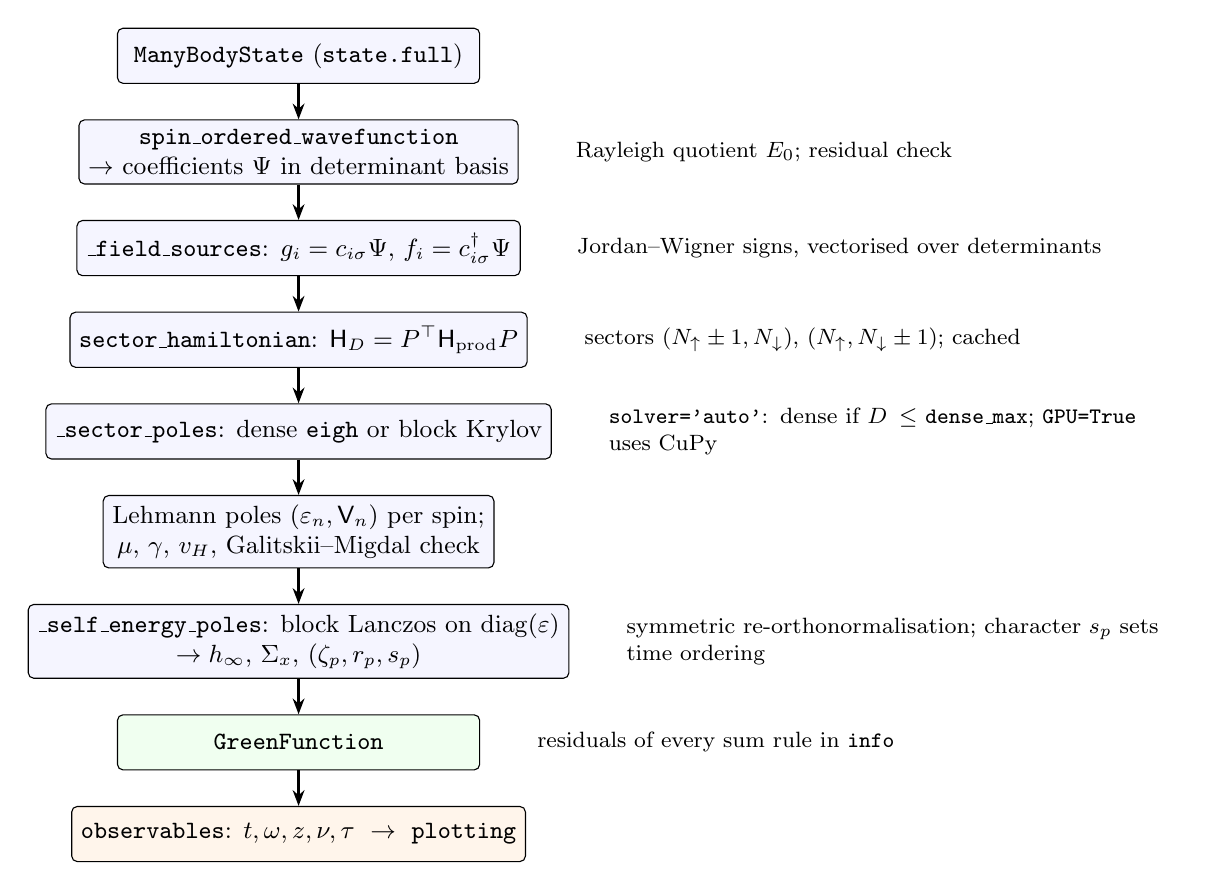
\begin{tikzpicture}[
  box/.style={draw,rounded corners=2pt,fill=blue!4,align=center,font=\small,minimum width=4.6cm,minimum height=7mm},
  note/.style={align=left,font=\footnotesize,text width=7.2cm},
  arr/.style={-{Stealth[length=2mm]},thick},
  node distance=4.5mm]
\node[box] (state) {\code{ManyBodyState} (\code{state.full})};
\node[box,below=of state] (psi) {\code{spin\_ordered\_wavefunction}\\ $\to$ coefficients $\Psi$ in determinant basis};
\node[box,below=of psi] (src) {\code{\_field\_sources}: $g_i=c_{i\sigma}\Psi$, $f_i=c^\dagger_{i\sigma}\Psi$};
\node[box,below=of src] (sec) {\code{sector\_hamiltonian}: $\mat H_D=P^\top\mat H_\text{prod}P$};
\node[box,below=of sec] (poles) {\code{\_sector\_poles}: dense \code{eigh} or block Krylov};
\node[box,below=of poles] (lehmann) {Lehmann poles $(\varepsilon_n,\mat V_n)$ per spin;\\ $\mu$, $\gamma$, $v_H$, Galitskii--Migdal check};
\node[box,below=of lehmann] (sigma) {\code{\_self\_energy\_poles}: block Lanczos on $\mathrm{diag}(\varepsilon)$\\ $\to h_\infty$, $\Sigma_x$, $(\zeta_p, r_p, s_p)$};
\node[box,below=of sigma,fill=green!6] (gf) {\code{GreenFunction}};
\node[box,below=of gf,fill=orange!8] (obs) {\code{observables}: $t,\omega,z,\nu,\tau$ $\;\to\;$ \code{plotting}};
\foreach \a/\b in {state/psi,psi/src,src/sec,sec/poles,poles/lehmann,lehmann/sigma,sigma/gf,gf/obs} \draw[arr] (\a) -- (\b);
\node[note,right=6mm of psi] {Rayleigh quotient $E_0$; residual check};
\node[note,right=6mm of src] {Jordan--Wigner signs, vectorised over determinants};
\node[note,right=6mm of sec] {sectors $(N_\up\pm1,N_\dn)$, $(N_\up,N_\dn\pm1)$; cached};
\node[note,right=6mm of poles] {\code{solver='auto'}: dense if $D\le$ \code{dense\_max}; \code{GPU=True} uses CuPy};
\node[note,right=6mm of sigma] {symmetric re-orthonormalisation; character $s_p$ sets time ordering};
\node[note,right=6mm of gf] {residuals of every sum rule in \code{info}};
\end{tikzpicture}
\caption{Data flow of \code{iDEA.methods.interacting.green\_function} and its consumers.}
\label{fig:flow}
\end{figure}

\subsection{The algorithm}

\Cref{lst:green} summarises \code{green\_function}, and \cref{lst:krylov} the shared block Krylov routine, which serves both the sector solve and the self-energy partition.

\begin{lstlisting}[style=pseudo,float=tbp,caption={\code{interacting.green\_function} (simplified).},label=lst:green,captionpos=b]
$\psi$ = spin_ordered_wavefunction(s, state)                    # checks $\sum|\psi|^2 = 1$
$\Psi$ = $\sqrt{N_\uparrow!N_\downarrow!}\,\psi$[determinants];  $E_0$ = $\langle\Psi|H_D|\Psi\rangle$;  check residual
for each spin $\sigma$:
    for removal ($c_{i\sigma}$) and addition ($c^\dagger_{i\sigma}$):
        $H$ = sector_hamiltonian(sector)                         # cached per sector
        $B$ = _field_sources($\Psi$, $\sigma$, create)              # $D\times N_x$
        $(E_n, \langle n|B\rangle)$ = dense eigh  or  block Krylov     # _sector_poles
        keep poles with weight $>10^{-14}$;  $\varepsilon_n = \pm(E_n - E_0)$;  $V$ = overlaps
$\mu$ = midgap over both spins (or None);  $\gamma_\sigma$, $n$, $v_H$ from removal poles
for each spin $\sigma$:
    $(h_\infty, \zeta, r, s)$ = _self_energy_poles($\varepsilon$, $V$, character)
    $\Sigma_x$ = $(h_\infty - h_0 - \mathrm{diag}(v_H))/\delta x$;   first-moment error = $\max|\Sigma_x - (-\gamma_\sigma v)|$
    warn about poles with $|s_p| < 10^{-6}$
Galitskii-Migdal error = $|E_{GM} - E_0|$;  return GreenFunction
\end{lstlisting}

\begin{lstlisting}[style=pseudo,float=tbp,caption={\code{interacting.\_block\_krylov(apply, B, max\_dim, tol, scale)}.},label=lst:krylov,captionpos=b]
$Q_1$ = left singular vectors of $B$ with $\sigma > \mathrm{tol}\cdot\sigma_\mathrm{max}$       # or $B$ itself if orthonormal
repeat:
    $W$ = apply($Q_\mathrm{last}$)                                  # $H_D Q$ (sparse) or $E\,Q$ (diagonal)
    if dimension reached: break
    $W \leftarrow W - Q(Q^\dagger W)$  twice                               # CGS2
    $Q_\mathrm{new}$ = left singular vectors of $W$ with $\sigma > \mathrm{tol}\cdot\mathrm{scale}$  # deflation
    if $Q_\mathrm{new}$ is empty: break                              # space exhausted: exact
$T = Q^\dagger (H Q)$, symmetrised;   return $T$, $Q$
\end{lstlisting}

\subsection{Diagnostics}

\code{GreenFunction.info} records:
\begin{itemize}
\item \code{rayleigh\_residual}: the Rayleigh residual of the state;
\item \code{sectors}: for each sector, the solver used, its dimension and its Krylov dimension;
\item \code{\{up,down\}\_completeness\_error}: $\max|\mat V\mat V^\dagger-1|$;
\item \code{\{up,down\}\_first\_moment\_error}: $\max|\Sigma_x-(-\gamma_\sigma v)|$;
\item \code{galitskii\_migdal\_error}: $|E_\text{GM}-E_0|$.
\end{itemize}
Every one of these should be at machine precision. A user can therefore check any calculation, including truncated Krylov runs, from \code{info} alone.

\subsection{Cost}

\begin{itemize}
\item \textbf{Building a sector.} This costs one sparse product $P^\top\mat H_\text{prod}P$, with $n_\up!\,n_\dn!$ non-zeros per column of $P$.
\item \textbf{Dense diagonalisation.} $O(D^3)$ time and $O(D^2)$ memory: $D=22\,801$ needs 4.2\,GB per double-precision copy.
\item \textbf{Block Krylov with $K$ vectors.} $O(K\,\mathrm{nnz}(\mat H_D) + DK^2)$ time and $2DK$ numbers of memory.
\item \textbf{The self-energy stage.} A spin channel with $M$ poles needs $O(M^3)$ time and $O(M^2)$ memory, on the CPU. This becomes the most memory-hungry step for the largest dense runs, with about 20\,GB for $M\approx23\,000$.
\item \textbf{Evaluation.} $O(\Nx^2 M)$ per time or frequency point.
\end{itemize}

\paragraph{Measured times.} On the container used for development (CPU only):
\begin{itemize}
\item hydrogen at $\Nx=\valNx$ (sectors of \valDimUp{} and \valDimDown{}, dense) takes \valTimeExact\,s;
\item a two-electron atom at $\Nx=41$ (sectors of 33\,620, Krylov dimension 1\,230) takes 17\,s;
\item the full test suite takes about 50\,s, and about 10\,s on the GitHub runner.
\end{itemize}

\subsection{Usage}

\Cref{lst:usage} shows a complete calculation.

\begin{lstlisting}[style=python,float=tbp,caption={Computing, evaluating and animating the exact $G$ and $\Sigma$ of the hydrogen atom, and the same calls for \GW{}.},label=lst:usage,captionpos=b]
import numpy as np, iDEA

x = np.linspace(-12, 12, 61)
v_int = iDEA.interactions.softened_interaction(x)
s = iDEA.system.System(x, -1.0 / (abs(x) + 1.0), v_int, "u")
state = iDEA.methods.interacting.solve(s, k=0)
green = iDEA.methods.interacting.green_function(s, state)  # solver="auto", GPU=False
print(green.info)                                           # sum-rule residuals

omega = np.linspace(-1.0, 2.0, 150)
G = iDEA.observables.green_function(s, green, omega=omega, eta=0.05)      # G(x,x';w)
S = iDEA.observables.self_energy(s, green, omega=omega)                   # Sigma_xc(x,x';w)
Sc_t = iDEA.observables.self_energy(s, green, t=np.linspace(0, 20, 200), part="c")
S_iw = iDEA.observables.self_energy(s, green, nu=np.linspace(0, 3, 50))   # z = mu + i nu
E = iDEA.observables.galitskii_migdal_energy(s, green)                    # equals state.energy

gw = iDEA.methods.mbpt.solve(s, mode="GW")                  # the same calls work for GW
S_gw = iDEA.observables.self_energy(s, gw, nu=np.linspace(0, 3, 50))
iDEA.plotting.animate_self_energy(s, green, omega=omega, spin="down",
                                  file_name="Sigma.mp4")
\end{lstlisting}

The hydrogen example runs end to end in the command-line script \path{tutorial/green_function_hydrogen.py} and in the notebook \path{tutorial/example_green_function.ipynb}. The script \path{report/make_figures.py} regenerates every figure and number in this report.

% ===========================================================================
\section{Testing and validation}
\label{sec:testing}

\paragraph{Before writing the code.} Every formula of \cref{sec:method} was first checked against an independent brute-force implementation in the full Fock space of small lattices. That implementation used explicit matrices for $c_i$ and $c_i^\dagger$ and covered:
\begin{itemize}
\item completeness;
\item the first moment;
\item Löwdin partitioning against direct Dyson inversion;
\item the Galitskii--Migdal energy for two and three electrons;
\item the Jordan--Wigner formulas.
\end{itemize}
All agreed to better than $4\times10^{-15}$. An independent review re-derived the whole pipeline in NumPy on small \code{u}, \code{ud}, \code{uu} and \code{du} grids, and found every sum rule to be at most $3\times10^{-15}$ and the hydrogen self-interaction identities at about $10^{-16}$.

\paragraph{The test suite.} The suite \code{tests/test\_green\_function.py} (\cref{tab:tests}) uses grids of 9--15 points, so that every sector can also be diagonalised completely. It covers:
\begin{itemize}
\item one electron (hydrogen, \code{u});
\item two electrons (a helium-like singlet, \code{ud});
\item an excited triplet with no gap (\code{uu});
\item three electrons (lithium-like, \code{uud}).
\end{itemize}
It runs in the continuous-integration workflow on every push. The 30 CPU tests pass, and the 2 GPU tests are skipped without CuPy.

\begin{table}[p]
\centering\small
\caption{The tests in \code{tests/test\_green\_function.py}.}
\label{tab:tests}
\begin{tabularx}{\textwidth}{>{\raggedright\arraybackslash}p{4.1cm}Yl}
\toprule
test & identity checked & tolerance \\
\midrule
\path{test_sum_rules} (u, ud, uu, uud) & Rayleigh residual, completeness, first moment ($\Sigma_x$ is Fock of exact $\gamma$), Galitskii--Migdal, $E_0$ & $10^{-10}$--$10^{-8}$ \\
\path{test_field_operators} & $\braket{g_i|g_j}=\gamma_{ji}\dx$, $\braket{f_i|f_j}=\delta_{ij}-\gamma_{ij}\dx$ (\cref{eq:source-identities}) & $10^{-12}$ \\
\path{test_density_matrix} & $G(t{=}0^-)=i\gamma$ and $G(\tau{=}0^-)=\gamma$ against \code{observables.density\_matrix} & $10^{-12}$ \\
\path{test_time_jump} & $G(0^+)-G(0^-) = -i\delta_{ij}/\dx$ & $10^{-8}$ \\
\path{test_galitskii_migdal} & \code{galitskii\_migdal\_energy} $=E_0$ (u, ud, uud) & $10^{-10}$ \\
\path{test_non_interacting_limit} & $v=0$: $\Sigma_{xc}=0$ and $G=G_0$ of \code{non\_interacting.solve} & $10^{-9}$ \\
\path{test_consistency_with_mbpt} & $v=0$: $G(i\nu)$, $G(\tau)$ equal \code{mbpt.non\_interacting\_green\_function} on its grids & $10^{-9}$ \\
\path{test_exhausted_krylov_is_exact} & Krylov with an exhausted space $=$ dense, for $G$ and $\Sigma$ & $10^{-9}$ \\
\path{test_truncated_krylov_moments} & three blocks: moments $0\ldots5$ exact, sum rules exact & $10^{-8}$ rel. \\
\path{test_poles_match_dyson} (ud, uu, uud) & pole-form $\Sigma_{xc}$ $=$ Dyson inversion at complex $z$ and retarded real $\omega$ & $10^{-9}$ \\
\path{test_matches_loewdin_partitioning} & $\Sigma_c$ $=$ Schur complement with a QR completion of $\mat V$ & $10^{-9}$ \\
\path{test_exchange_is_fock} & $\Sigma_x$ $=$ \code{observables.exchange\_potential} of exact $\gamma$ & $10^{-9}$ \\
\path{test_time_ordering} (ud, uu) & $\sgn\mathrm{Im}\braket{r_p|\Sigma^T_\text{Dyson}(\zeta_p)|r_p} = -\sgn s_p$ for isolated poles & sign \\
\path{test_hydrogen_self_interaction} & single removal pole at $E_0$; $(v_H+\Sigma_x)\phi=0$; $\Sigma_c(z)\phi=0$; all $s_p=+1$ & $10^{-9}$ \\
\path{test_imaginary_time_matches_fourier_transform} & $G(\tau)$ $=$ \code{SpaceTimeGrid} transform of $G(i\nu)$ & $10^{-6}$ \\
\path{test_quasiparticle_state} & a \GW{} state passes through \code{green\_function}, \code{self\_energy} & $10^{-6}$ \\
\path{test_errors} & invalid axes and parts; no gap $\Rightarrow$ $\mu$ is \code{None} and \code{nu} is refused & raises \\
\path{test_invalid_solver} & unknown solver & raises \\
\path{test_normalisation} & $\int A(x,x;\omega)\,d\omega\,\dx = 1$ & $5\times10^{-3}$ \\
\path{test_matches_retarded_green_function} & $A = \tfrac{i}{2\pi}(G^R-G^{R\dagger})$ & $10^{-12}$ \\
\path{test_animations} & \code{.gif} written for $G(\omega)$ and $\Sigma_c(t)$; snapshot; invalid input & runs \\
\path{test_gpu_matches_cpu} (dense, Krylov) & GPU $=$ CPU for $G$ and $\Sigma$ (skipped without CuPy) & $10^{-9}$ \\
\bottomrule
\end{tabularx}
\end{table}

\paragraph{The production example.} The hydrogen calculation of \cref{sec:results} ($\Nx=\valNx$) reports:
\begin{itemize}
\item a Rayleigh residual of $\valRayleigh$;
\item a completeness error of $\valCompleteness$;
\item a first-moment error of $\valFirstMoment$;
\item a Galitskii--Migdal error of $\valGMError$;
\item $\Vert(v_H+\Sigma_x)\phi\Vert_\infty = \valSigmaXResidual$.
\end{itemize}

% ===========================================================================
\section{Illustrative results: the one-dimensional hydrogen atom}
\label{sec:results}

\paragraph{The system.} One spin-up electron in $v_\text{ext}=-1/(|x|+1)$, with the softened interaction $v(x,x')=1/(|x-x'|+1)$, on $\Nx=\valNx$ points in $[-\valLength,\valLength]$ ($\dx=\valDx$). The exact ground-state energy is $E_0=\valEzero$. The midgap chemical potential is $\mu=\valMu$. The spin-up and spin-down channels have \valPolesUp{} and \valPolesDown{} poles. Every number in this section is regenerated by \code{report/make\_figures.py} (\cref{app:production}).

\paragraph{Spectral functions (\cref{fig:spectral}).} In the spin-up channel, the single removal pole at $E_0$ carries the whole occupied orbital. In the spin-down channel, an electron added to the atom can bind as H$^-$: there is an addition pole at $\valHminus$, just below the continuum, so the electron affinity is $\valEAffinity$. Above it, the box states of the continuum appear as the regular pattern of standing waves.

\begin{figure}[t]
\centering
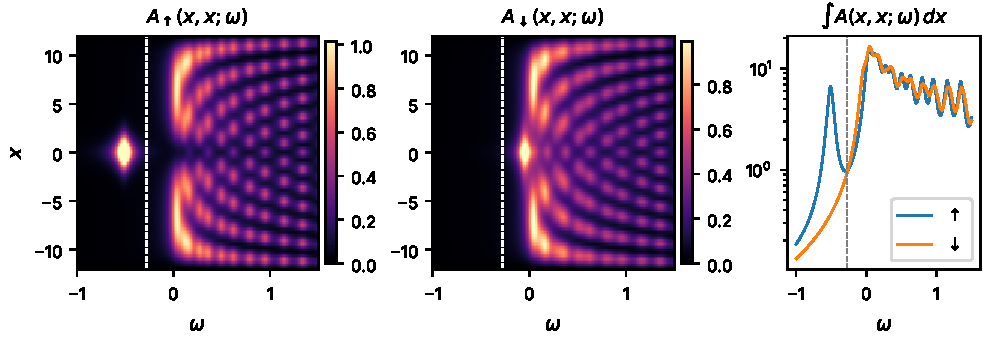
\includegraphics[width=\textwidth]{figures/spectral_functions.pdf}
\caption{Local spectral functions $A_\sigma(x,x;\omega)$ of the hydrogen atom ($\eta=0.05$) and their traces. The dashed line marks $\mu$. Spin up: the removal pole at $E_0$ and the triplet continuum. Spin down: the singlet continuum, with the H$^-$ bound state at its threshold.}
\label{fig:spectral}
\end{figure}

\paragraph{Self-interaction and self-screening (\cref{fig:screening}, \cref{tab:energies}).} The exact $\Sigma_{c\up}(\mu+i\nu)$ annihilates the occupied orbital to $\valScreeningExact$ at every frequency (\cref{sec:one-electron}). G$_0$W$_0$@HF, GW$_0$ and self-consistent \GW{} leave residuals of $\valScreeningGzWz$, $\valScreeningGWz$ and $\valScreeningGW$: the self-screening error~\cite{nelson2007,wetherell2018}. In energy terms, every \GW{} variant overbinds the electron, both in the total energy and in the ionisation energy.

\begin{figure}[t]
\centering
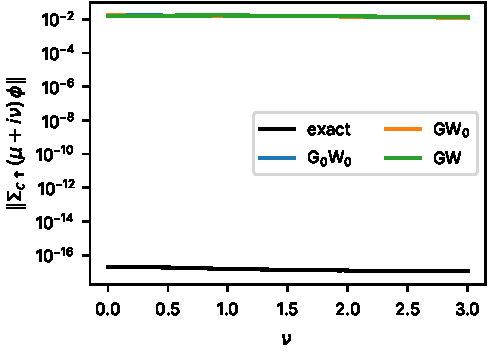
\includegraphics[width=0.52\textwidth]{figures/self_screening.pdf}
\caption{Self-screening: $\Vert\Sigma_{c\up}(\mu+i\nu)\phi\Vert$ for the exact self-energy (black; machine zero) and for \GW{} at three levels of self-consistency, each with its own occupied orbital.}
\label{fig:screening}
\end{figure}

\begin{table}[t]
\centering\small
\caption{Hydrogen at $\Nx=\valNx$: total (Galitskii--Migdal) energies and removal energies. For \GW{}, the removal energy is the static quasiparticle energy of the occupied state.}
\label{tab:energies}
\begin{tabular}{lrr}
\toprule
method & total energy & removal energy \\
\midrule
exact & $\valEzero$ & $\valEzero$ \\
G$_0$W$_0$@HF & $\valEGzWz$ & $\valEpsGzWz$ \\
GW$_0$ & $\valEGWz$ & $\valEpsGWz$ \\
\GW{} & $\valEGW$ & $\valEpsGW$ \\
\bottomrule
\end{tabular}
\end{table}

\paragraph{The static correlation self-energy (\cref{fig:static}).} The full two-point structure of $\Sigma_c(x,x';\mu+i0)$ is shown in \cref{fig:static}.
\begin{itemize}
\item \textbf{Spin up.} The exact $\Sigma_{c\up}$ is not zero. It acts only in the space orthogonal to $\phi$, and correlates a second spin-up electron with the first. Its most negative element is $\valDepthExactUp$, half that of \GW{} ($\valDepthGWUp$). The \GW{} $\Sigma_{c\up}$ differs from it near the nucleus, where the occupied orbital lives. This difference is the self-screening of \cref{fig:screening}.
\item \textbf{Spin down.} The exact $\Sigma_{c\dn}$ is the polarisation potential felt by an added spin-down electron. Its most negative element is $\valDepthExactDown$, against $\valDepthGWDown$ in \GW{}.
\end{itemize}
Both self-energies are concentrated near the diagonal and within a few units of the nucleus. This is a first glimpse of the nearsightedness that the research proposal sets out to quantify.

\begin{figure}[t]
\centering
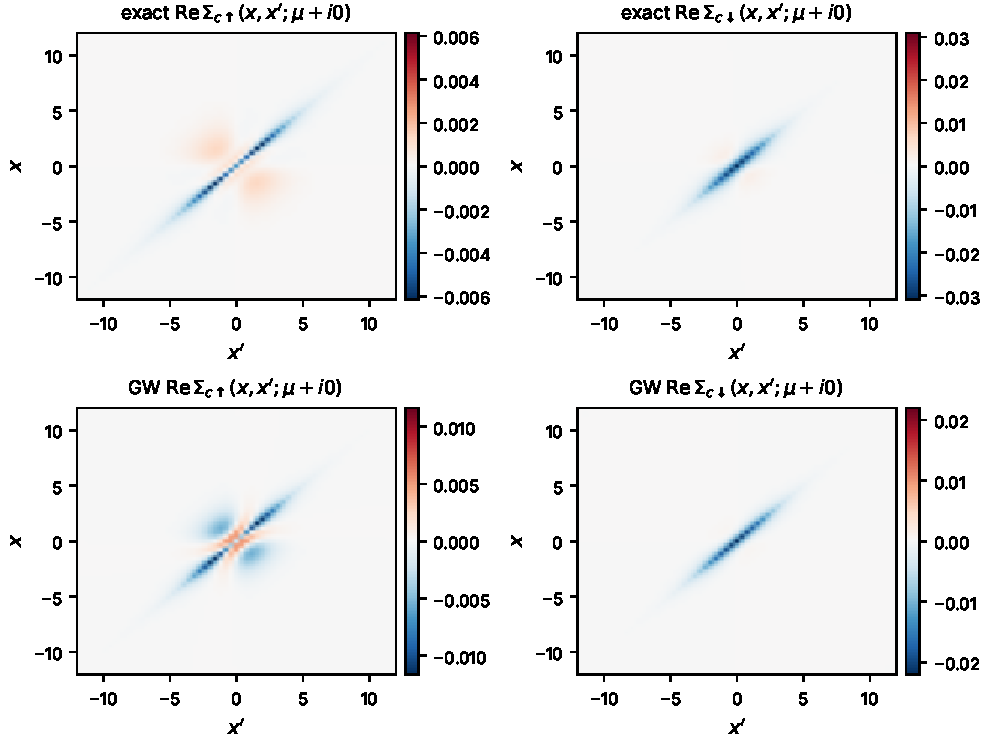
\includegraphics[width=\textwidth]{figures/static_correlation.pdf}
\caption{$\mathrm{Re}\,\Sigma_c(x,x';\mu+i0)$ for both spins, exact (top) and self-consistent \GW{} (bottom). Each panel has its own symmetric colour scale.}
\label{fig:static}
\end{figure}

\paragraph{Two-point structure on the real axis (\cref{fig:frames}).} The two rows show different things:
\begin{itemize}
\item \textbf{Top: $G_\dn$ at the H$^-$ pole.} At $\omega=\valHminus$, $\mathrm{Im}\,G_\dn$ is dominated by $-d\,d^\dagger/\eta$. It is a picture of the H$^-$ Dyson orbital: diffuse, but bound.
\item \textbf{Bottom: $\Sigma_{xc\dn}$ at $\omega=0.5$, in the continuum.} The imaginary part is non-zero. An electron added at this energy can scatter into configurations in which the bound electron is excited.
\end{itemize}
These are single frames of the videos produced by \path{animate_green_function} and \path{animate_self_energy}.

\begin{figure}[t]
\centering
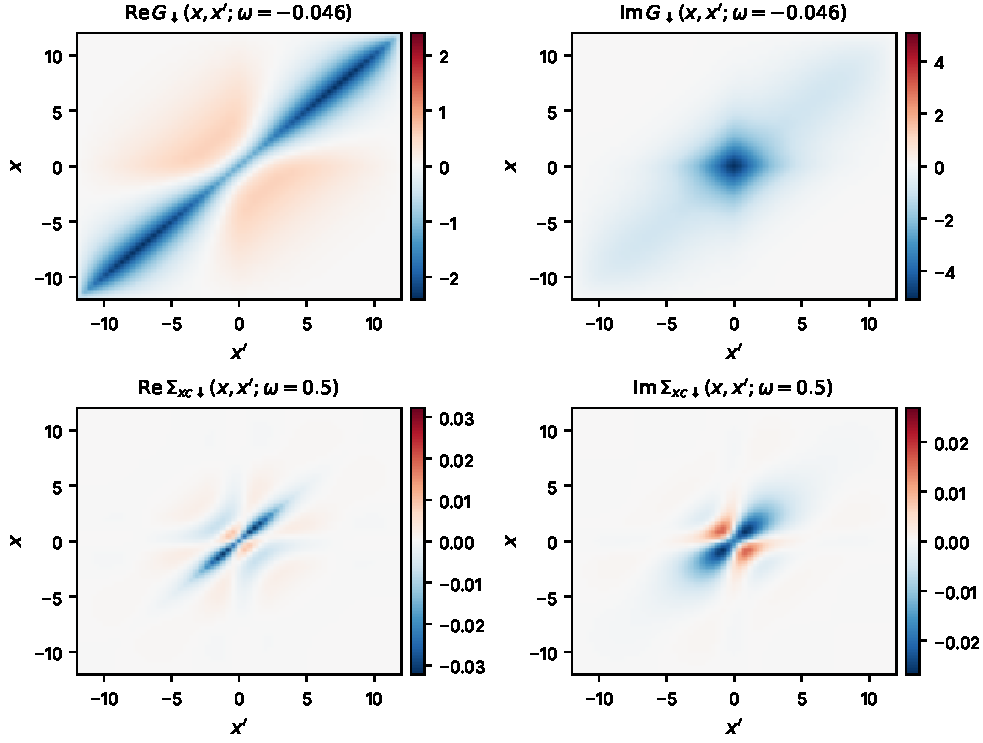
\includegraphics[width=\textwidth]{figures/frequency_frames.pdf}
\caption{Top: $G_\dn(x,x';\omega)$ at the H$^-$ addition pole. Bottom: $\Sigma_{xc\dn}(x,x';\omega=0.5)$ in the continuum ($\eta=0.05$).}
\label{fig:frames}
\end{figure}

\paragraph{An electron injected at the nucleus (\cref{fig:injected}).} The column $G(x,0;t>0)$ is the amplitude of an electron injected at $x'=0$, here band-limited with \code{cutoff=0.5} (\cref{sec:visualisation}). The two spins behave very differently:
\begin{itemize}
\item \textbf{Spin up.} Pauli exclusion projects $\phi$ out of the injected electron. This leaves a hole at the nucleus, and the amplitude starts in two lobes. With no bound triplet state, it flies away, and it returns only after reflecting off the box.
\item \textbf{Spin down.} Part of the amplitude binds as H$^-$ and stays at the atom, while the rest radiates away.
\end{itemize}

\begin{figure}[t]
\centering
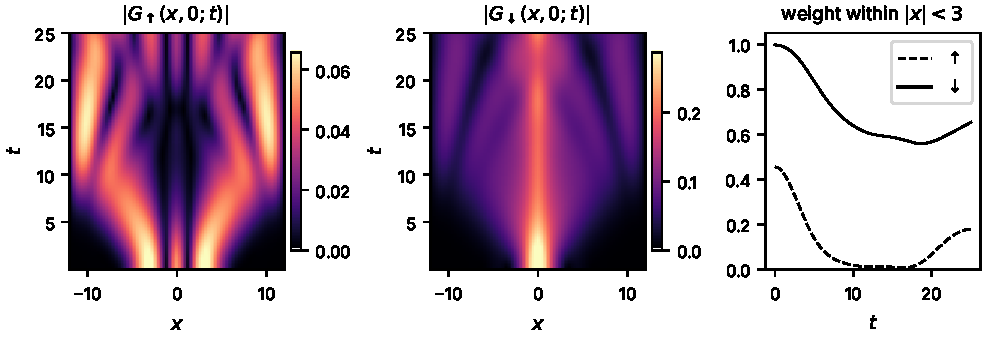
\includegraphics[width=\textwidth]{figures/injected_electron.pdf}
\caption{An electron injected at the nucleus: $|G_\sigma(x,0;t)|$ for spin up and spin down (band-limited with \code{cutoff=0.5}), and the fraction of $|G|^2$ within $|x|<3$.}
\label{fig:injected}
\end{figure}

% ===========================================================================
\section{Limitations and outlook}
\label{sec:limitations}

\begin{itemize}
\item \textbf{System size.} The method is exact but its cost grows exponentially with $N$. With dense sectors, one electron is routine on fine grids, and two electrons on coarse ones. Block Krylov extends two-electron systems to grids of about 100 points ($N+1=3$), and three electrons to coarser grids.
\item \textbf{The self-energy stage.} It runs on the CPU, with $O(M^3)$ time and $O(M^2)$ memory in the number of poles $M$. A GPU version of this step is a natural extension.
\item \textbf{Truncated Krylov.} The pole positions change, but the low moments do not (\cref{sec:krylov}). Properties that depend on fine spectral detail far from $\mu$ need convergence checks in \code{krylov\_dim}.
\item \textbf{Visualisation filter.} \code{cutoff} is for visualisation only and is not exact.
\item \textbf{States without a gap.} For states with no gap, such as excited states, $\mu$ is \code{None}, and imaginary-axis evaluation needs an explicit $z$.
\item \textbf{Hedin's other functions.} The exact polarisability $P$ and screened interaction $W$ are not constructed. Only $G$ and $\Sigma_{xc}$ are.
\end{itemize}

\paragraph{Next steps.} These follow the research proposal:
\begin{enumerate}
\item production runs on a GPU (\cref{app:production});
\item two-electron atoms and stretched H$_2$-like molecules, where $\Sigma$ develops strong-correlation structure;
\item a quantitative study of the nearsightedness of the exact $\Sigma(x,x';\omega)$ compared with \GW{} and with exact Kohn--Sham potentials~\cite{wetherell2019}.
\end{enumerate}

% ===========================================================================
\appendix
\section{Production calculations on an RTX 4090}
\label{app:production}

These are the runs that were too large for the development container. Install CuPy first with \code{pip install -e ".[gpu]"}.

\begin{enumerate}
\item \textbf{GPU tests.} The GPU paths have not yet been run on hardware.
\begin{lstlisting}
pytest tests/test_green_function.py tests/test_gpu.py -v
\end{lstlisting}
\item \textbf{Production hydrogen, with videos.}
\begin{lstlisting}
python tutorial/green_function_hydrogen.py --nx 151 --dense-max 30000 --gpu --out hydrogen_151
\end{lstlisting}
\begin{itemize}
\item The sectors are $(2,0)$ with $D=11\,325$ and $(1,1)$ with $D=22\,801$. Both are diagonalised densely on the GPU, at about 4.2\,GB per copy of the larger matrix; \code{eigh} needs a few copies.
\item The self-energy stage then runs on the CPU, using about 20\,GB of RAM.
\item $\Nx=161$ ($D=25\,921$) should also fit, but it is tight in 24\,GB.
\end{itemize}
\item \textbf{This report at production resolution.}
\begin{lstlisting}
python report/make_figures.py --nx 151 --dense-max 30000 --gpu
make -C report/latex
\end{lstlisting}
This rewrites \code{report/latex/figures/*.pdf} and \code{values.tex}, so every figure and number in \cref{sec:testing,sec:results} updates.
\item \textbf{Convergence.} Repeat at \code{--nx 101}, and with \code{--length 20}, to converge the diffuse H$^-$ state. A larger box also delays the reflections in \cref{fig:injected}.
\item \textbf{Optional: two electrons with Krylov.} The $(2,1)$ and $(1,2)$ sectors have $D=510\,050$ at $\Nx=101$:
\begin{lstlisting}[style=python]
x = np.linspace(-10, 10, 101)
s = iDEA.system.System(x, -2.0 / (abs(x) + 1.0), iDEA.interactions.softened_interaction(x), "ud")
state = iDEA.methods.interacting.solve(s, k=0, GPU=True)
green = iDEA.methods.interacting.green_function(s, state, krylov_dim=1500, GPU=True)
print(green.info)
\end{lstlisting}
With $K=1500$, the Krylov basis and its image take about 12\,GB on the GPU.
\end{enumerate}

Please send back \code{info.json} (or \code{green.info}), the rebuilt \code{report.pdf} and the best videos.

% ===========================================================================
\section{Derivations}
\label{app:derivations}

\subsection{Normalisation of the spin-ordered wavefunction}
\label{app:spin-ordered}

$\Psi$ is antisymmetric under exchange of space--spin pairs and normalised as $\sum_{\{x\sigma\}}|\Psi|^2\dx^N = 1$. For each spatial configuration, the spin labels take one of $\binom{N}{N_\up}$ placements of the up spins among the $N$ electrons. Any placement can be brought to the canonical one (ups first) by a permutation of electrons, which changes only the sign. So each placement carries the same weight, $1/\binom{N}{N_\up}$ of the total, and \cref{eq:spin-ordered} is normalised.

The determinant coefficient $\braket{\mathbf a;\mathbf b|\Psi}$ collects the $n_\up!\,n_\dn!$ equal-magnitude orderings of an ordered configuration. With the $1/\sqrt{n_\up!n_\dn!}$ normalisation of the antisymmetrised determinant, this gives the factor $\sqrt{n_\up!\,n_\dn!}$.

\subsection{Jordan--Wigner signs}

In $\ket{\mathbf a;\mathbf b}$, all up operators stand to the left of all down operators, each group in increasing site order. To annihilate $c^\dagger_{a_k\up}$, the operator $c_{a_k\up}$ is anticommuted past the $k-1$ up operators to its left, which gives $(-1)^{k-1}$. To annihilate $c^\dagger_{b_k\dn}$, it is anticommuted past all $n_\up$ up operators and the $k-1$ down operators before it, which gives $(-1)^{n_\up+k-1}$. The test of \cref{eq:source-identities} checks both the signs and the normalisation.

\subsection{The first moment and the exact Fock operator}
\label{app:first-moment}

From the Lehmann representation, $\sum_n\varepsilon_n\mat V_{in}\mat V_{jn}^* = \braket{\{[c_{i\sigma},\hat H],c^\dagger_{j\sigma}\}}$. For the Hamiltonian of \cref{sec:method}, $[c_{i\sigma},\hat H] = \sum_k(\mat h_0)_{ik}c_{k\sigma} + \sum_{k\sigma'}v_{ik}\hat n_{k\sigma'}c_{i\sigma}$. The anticommutator with $c^\dagger_{j\sigma}$ gives
\begin{equation}
(\mat h_0)_{ij} + \delta_{ij}\sum_{k}v_{ik}\braket{\hat n_k} - v_{ij}\braket{c^\dagger_{j\sigma}c_{i\sigma}}
= (\mat h_0)_{ij} + \delta_{ij}v_H(x_i) - v(x_i,x_j)\gamma_\sigma(x_i,x_j)\,\dx,
\end{equation}
which is $h_\infty\dx$ of \cref{eq:hinf}. The Hartree term contains the total density, and the Fock term the same-spin density matrix. The Fock term exactly removes the self-interaction contained in the Hartree term.

\subsection{Galitskii--Migdal in Lehmann form}

For a removal pole, $\varepsilon_m = E_0 - E_m$. Since $\hat H\ket{\Psi_0} = E_0\ket{\Psi_0}$, we have $(E_0-\hat H)c_{i\sigma}\ket{\Psi_0} = [c_{i\sigma},\hat H]\ket{\Psi_0}$, so
\begin{equation}
\sum_{m}\varepsilon_m\,\mat V_{im}^*\mat V_{im} = \braket{\Psi_0|c^\dagger_{i\sigma}[c_{i\sigma},\hat H]|\Psi_0}.
\end{equation}
Summing over $i$ and $\sigma$ with the commutator of \cref{app:first-moment} gives $\braket{\hat H_1} + 2\braket{\hat V}$, where $\hat H_1$ is the one-body part and $\hat V$ the interaction. Similarly, $\sum_{i\sigma}\sum_m\mat V_m^\dagger\mat h_0\mat V_m = \braket{\hat H_1}$. Half the sum of the two is $\braket{\hat H_1}+\braket{\hat V} = E_0$, which is \cref{eq:gm}~\cite{galitskii1958,fetter1971}. The code evaluates exactly this, $E = \tfrac12\sum_\sigma\sum_m[\mat V_m^\dagger\mat h_0\mat V_m + \varepsilon_m\Vert\mat V_m\Vert^2]$.

% ===========================================================================
\bibliographystyle{unsrtnat}
\bibliography{refs}

\end{document}
